\documentclass[11pt]{article}
\usepackage[margin=1in]{geometry}
\usepackage{amsmath}
\usepackage{amssymb}
\usepackage{graphicx}
\usepackage{booktabs}
\usepackage{float}
\usepackage{caption}
\usepackage[hidelinks]{hyperref}

\graphicspath{{../results/2026-10-15_psd-d2-ln-mass/}}
\newcommand{\tabdir}{../results/2026-10-15_psd-d2-ln-mass/tex}

\newcommand{\tsec}{t^*_{\mathrm{sec}}}
\newcommand{\ttau}{t^*_{\tau}}
\newcommand{\dd}{\mathrm{d}}
\captionsetup{font=small, labelfont=bf}

\title{The Power Spectrum of $\dd^2 \ln M/\dd t^2$\\ and the Characteristic Time}
\date{20 October 2026}
\author{}

\begin{document}
\maketitle

\begin{abstract}
\noindent
We compute the power spectral density (PSD) of $g(t) = \dd^2\ln M/\dd t^2$, where
$M(t)$ is the total mass, locate its peak, and relate it to both definitions of the
characteristic time $t^*$ the project has used. The results:
\begin{enumerate}
\item \textbf{The value of the PSD at $f=0$ is exactly $\lambda^2$}, where
  $\lambda$ is the asymptotic decay rate of $M$. That is, $S(0) = (\ln 10 \times
  \text{fit slope})^2$, the slope either kernel records.
\item \textbf{When the escape rate rises monotonically ($g\le 0$), the PSD peaks
  at $f=0$.} This is a theorem, observed in all 49 runs of a sweep with $a=b$.
\item \textbf{The original $t^*$} (the secant through $\log_{10}M$ at $t=0.4,0.5$)
  \textbf{is exactly the centroid of $g$} once $g$ is weighted by the fit window.
  In the spectrum it appears as the phase slope at $f=0$. A PSD discards phase, so
  it cannot contain this $t^*$. Across the sweep the PSD's half-power frequency
  tracks it empirically, $t^*\approx 0.194\,f_{1/2}^{-0.683}$, with 1.6\% scatter.
\item \textbf{The current $t^*$} (the right sweep of $|g|\le\tau$) \textbf{is set
  by the slowest transient mode of $g$'s tail}, $g\sim Ce^{-\gamma t}\cos\omega t$.
  For a real mode $t^*_\tau = \ln(C/\tau)/\gamma$, and for a complex one it falls
  within half a period of that. So $t^*_\tau$ moves by $\ln 10/\gamma$ per decade
  of $\tau$.
\item \textbf{With slow switching onto the advective layer ($b\le1$), $g$ changes
  sign and the PSD peaks at $f>0$}, reaching up to $14\,S(0)$. That peak is the
  frequency $\omega/2\pi$ of the tail mode only for $a\le1$. For larger $a$ it
  comes from a biphasic early pulse and sits up to $3\times$ higher, so the PSD
  peak is not by itself a reliable handle on $t^*_\tau$.
\end{enumerate}
\end{abstract}

\section{Definitions}

\paragraph{Mass, escape rate and $g$.}
$M(t)$ is the total mass, diffusive plus advective layer, with $M(0)=1$. Write
\[
  \ell(t)=\ln M(t),\qquad \kappa(t)=-\ell'(t),\qquad g(t)=\ell''(t)=-\kappa'(t).
\]
$\kappa$ is the escape rate per surviving particle (the hazard rate), and $g$ is
minus its rate of change. At late times one mode dominates, so
$\ell\to\alpha-\lambda t$ and $\kappa\to\lambda$. With the centred initial
condition no mass sits on the absorbing boundary at $t=0$, so $\kappa(0)=0$.

\paragraph{The two characteristic times.}
\begin{itemize}
\item $\tsec$, the original definition, in force until 28 September 2026 and used
  by the 2026-08-18 grid study. Fit a secant to $\log_{10}M$ through $x_1=0.4$ and
  $x_2=0.5$, and take $\tsec$ to be where it crosses $\log_{10}M=0$.
\item $\ttau$, the current definition (\texttt{launch.\_char\_time\_onset}). With
  $g$ taken as a second difference at spacing $H\approx10^{-4}$, $\ttau$ is the
  first sample after the last one with $|g|>\tau$. The default is $\tau=10^{-3}$;
  the 96$^2$ study used $\tau=10^{-2}$.
\end{itemize}
Both are functionals of $g$. The analysis began against $\tsec$, which was the
kernel in this working copy at the time. The current definition was merged
afterwards, and Section~\ref{sec:ab} treats it on the configuration of the current
studies.

\paragraph{The spectrum.}
$g$ is a transient, not a stationary signal, so its PSD is the energy spectral
density
\[
  S(f)=|G(f)|^2,\qquad G(f)=\int_0^\infty g(t)\,e^{-2\pi i f t}\,\dd t ,
\]
evaluated on $f\ge0$. A periodogram differs from it only by the constant factor
$1/T$, which moves no peak.

\section{Exact results}

\subsection{The zero-frequency value: $S(0)=\lambda^2$}
Integrate $g$ once:
\[
  G(0)=\int_0^\infty g\,\dd t=\ell'(\infty)-\ell'(0)=-\lambda+\kappa(0)=-\lambda .
\]
Hence $S(0)=\lambda^2=(\ln 10\times\text{fit slope})^2$. This holds for the slope
of the old secant and for the current kernel's least-squares slope over
$[\ttau,T]$, because both measure the same asymptotic $\lambda$ once $g$ has
decayed.

\subsection{The original $t^*$ is the centroid of $g$}
Write $\ell=\alpha-\lambda t+u$, where $u$ and $u'$ go to zero at large $t$, so
that $u''=g$. Integrating by parts,
\[
  \int_0^\infty t\,g\,\dd t=\big[t\,u'\big]_0^\infty-\int_0^\infty u'\,\dd t=u(0)=\ell(0)-\alpha=-\alpha .
\]
Once the secant lies on the asymptote, $\tsec=\alpha/\lambda$. Dividing the two
integrals,
\begin{equation}
  \tsec=\frac{\int_0^\infty t\,g\,\dd t}{\int_0^\infty g\,\dd t},
  \label{eq:centroid}
\end{equation}
which is the centroid of $g$.

\paragraph{The exact finite-window form.}
This form needs no late-time assumption. Because $\ell(0)=\ell'(0)=0$, we can
write $\ell(x)=\int_0^x(x-s)\,g(s)\,\dd s$. Substituting this into the secant's
zero, $\tsec=(x_1\ell_2-x_2\ell_1)/(\ell_2-\ell_1)$, gives
\begin{equation}
  \tsec=\frac{\int_0^{x_2}\min(s,x_1)\,w(s)\,g(s)\,\dd s}{\int_0^{x_2}w(s)\,g(s)\,\dd s},
  \qquad
  w(s)=\begin{cases}1 & s\le x_1,\\ \frac{x_2-s}{x_2-x_1} & x_1<s\le x_2,\\ 0 & s>x_2.\end{cases}
  \label{eq:window}
\end{equation}
If $g$ has died out before $x_1$, then $w=1$ wherever $g\neq0$ and
\eqref{eq:window} reduces to \eqref{eq:centroid}.

The denominator of \eqref{eq:window} is the secant slope times $\ln 10$, which is
always negative. So \textbf{$\tsec<0$ exactly when the positive part of $g$
inside the window, weighted by $\min(s,x_1)\,w(s)$, outweighs the negative
part.} That condition is met when the escape rate overshoots and a large positive
lobe of $g$ follows the initial negative pulse. Section~\ref{sec:ab} finds this
for the same four $(a,b)$ pairs that the 96$^2$ study found to have negative
$\tsec$.

\paragraph{In the spectrum.} Expanding $G$ at low frequency,
\[
  G(f)=-\lambda\Big[1-2\pi i f\,\tsec-\tfrac{(2\pi f)^2}{2}\mu_2+\dots\Big],
  \qquad \mu_2=\frac{\int t^2g}{\int g}.
\]
So $\tsec$ is the group delay of $G$ at zero frequency,
$\tsec=-(1/2\pi)\,\dd\arg G/\dd f|_{f=0}$. The magnitude obeys
$S(f)=\lambda^2[1-(2\pi f)^2\sigma^2+O(f^4)]$ with $\sigma^2=\mu_2-{\tsec}^2$:
the curvature at $f=0$ gives the spread of $g$, not its position.

\subsection{Where the PSD peaks}
If $g\le0$ everywhere (the escape rate rises monotonically), the triangle
inequality gives
\[
  |G(f)|\le\int_0^\infty|g|\,\dd t=\Big|\int_0^\infty g\,\dd t\Big|=|G(0)|,
\]
with equality only at $f=0$. \textbf{The maximum is then at $f=0$, with height
$\lambda^2$.} More generally, let $p=\int g^+/\int|g|$ be the fraction of $g$'s
weight that is positive. The same inequality bounds how far the PSD can rise
above its zero-frequency value:
\begin{equation}
  \frac{\max_f S(f)}{S(0)}\le\frac{1}{(1-2p)^2}.
  \label{eq:bound}
\end{equation}
A peak away from $f=0$ therefore requires $g$ to change sign.

\subsection{What a PSD cannot hold}
Shifting $g$ in time by $\tau_0$ multiplies $G$ by $e^{-2\pi i f\tau_0}$. That
leaves $S$ unchanged and shifts every absolute time, including $\tsec$, by
$\tau_0$. Absolute times are therefore carried only by the phase of $G$, never by
the PSD. Any link between the PSD and a characteristic time goes through the
\emph{shape} of $g$: its width, or its tail modes.

\subsection{The current $t^*$ and the tail modes of $g$}
\label{sec:tail}
Suppose late-time decay is a sum of modes, $M=\sum_k c_ke^{-\lambda_kt}$, with
$\lambda_1$ real and slowest. Then
$\ell=\ln c_1-\lambda_1t+\ln(1+\varepsilon)$, where
$\varepsilon=\sum_{k\ge2}(c_k/c_1)e^{-(\lambda_k-\lambda_1)t}$, so
$g=\varepsilon''+O(\varepsilon^2)$. Let $\Delta=\lambda_2-\lambda_1=\gamma\pm i\omega$
be the slowest correction. Then
\[
  g(t)\simeq C\,e^{-\gamma t}\cos(\omega t+\phi),\qquad
  C=2\left|\tfrac{c_2}{c_1}\right||\Delta|^2\ \text{(complex pair)},\quad
  C=\left|\tfrac{c_2}{c_1}\right|\Delta^2\ \text{(real, }\omega=0).
\]
The right sweep finds the last time $|g|$ exceeds $\tau$. Let
$t_{\rm env}=\ln(C/\tau)/\gamma$ be the time at which the envelope falls to
$\tau$.
\begin{itemize}
\item For a real mode, $|g|$ decays monotonically, so $\ttau=t_{\rm env}$.
\item For a complex mode, $|g|$ has lobes spaced $\pi/\omega$ apart, so the last
  lobe above $\tau$ ends within about half a period before the envelope crossing:
  $t_{\rm env}-\pi/\omega\lesssim\ttau\le t_{\rm env}$.
\end{itemize}
Either way, on average
\begin{equation}
  \frac{\dd\ttau}{\dd\ln(1/\tau)}=\frac{1}{\gamma}.
  \label{eq:tausens}
\end{equation}
In the spectrum, this mode contributes poles at $2\pi f=\pm\omega+i\gamma$: a
resonance at $f=\omega/2\pi$ with half-width $\gamma/2\pi$. The resonance is the
PSD's maximum only if it outweighs the broadband contribution of $g$'s early
pulse.

\subsection{Continuum check}
Take pure diffusion from a point source at the centre of the unit disc, with an
absorbing rim and $D=1$. Then $M=\sum_nc_ne^{-j_n^2t}$, with $j_n$ the zeros of
$J_0$ and $c_n=2/(j_nJ_1(j_n))$. The prediction is $\tsec=\ln c_1/j_1^2=0.081484$.
From the series, the centroid of $g$ is $0.081484$ and $\sqrt{S(0)}=5.783186=j_1^2$,
both as predicted. Here $g\le0$ throughout, the PSD peaks at $f=0$, and
$f_{1/2}=3.624$.

\section{Method}
Every solve runs the project's CPU solver through \texttt{launch.\_solve\_mass\_analysis},
the path the characteristic-time kernels use. The mass series is kept at the
kernel's sampling, one sample per 5 time steps. Both definitions of $t^*$ are
recomputed from that series: $\tsec$ by the secant, and $\ttau$ by calling
\texttt{launch.\_char\_time\_onset} itself.

As cross-checks, the $N=16$ grid-study configuration gives $\tsec=0.052357$,
$0.055390$ and $0.057689$ at $48^2$, $64^2$ and $80^2$. Each matches the published
grid study.

\begin{itemize}
\item \textbf{Differencing.} $M$ is sampled every $10^{-5}$ or less, far finer than
  any feature of $\ln M$, so differencing at that spacing only amplifies
  round-off. We keep every $k$-th sample to reach a spacing of
  $\approx2\times10^{-5}$ (exact, with no filtering) and then take central
  differences. The moments $\int g$ and $\int tg$ are computed by integrating by
  parts from $\ell$ and $\ell'$, so noise in $g$ cannot bias them.
\item \textbf{Spectrum.} $G$ is computed by FFT with $16\times$ zero padding. The
  half-power frequency $f_{1/2}$ is the first $f$ with $S(f)\le S(0)/2$.
\item \textbf{Tail modes.} $\gamma$, $\omega$ and $C$ come from a matrix-pencil
  fit of $g$ on the window between $\ttau(\tau=3\times10^{-2})$ and
  $\ttau(\tau=10^{-4})$. We keep the slowest-decaying pole whose amplitude is not
  negligible. Separately, $\gamma_\tau$ is the inverse slope of $\ttau$ against
  $\ln(1/\tau)$ over 25 values of $\tau$ in $[10^{-4},3\times10^{-2}]$, which
  tests \eqref{eq:tausens}.
\end{itemize}

\section{Results I: fast switching, $a=b$}

The sweep has 48 runs at $32^2$: $N\in\{4,8,16\}$, $v\in\{10,10^2,10^3,10^4\}$ and
$a=b\in\{1,10,10^2,10^3\}$, each run to $T=2$, plus one pure-diffusion run (one
microtubule, $a=b=v=0$). In every run $g$ is essentially a single negative pulse;
only two runs have any positive part, and it is at most 1.3\% of $\int|g|$. The PSD peaks at $f=0$
throughout, as the theorem requires.

\begin{figure}[H]
\centering
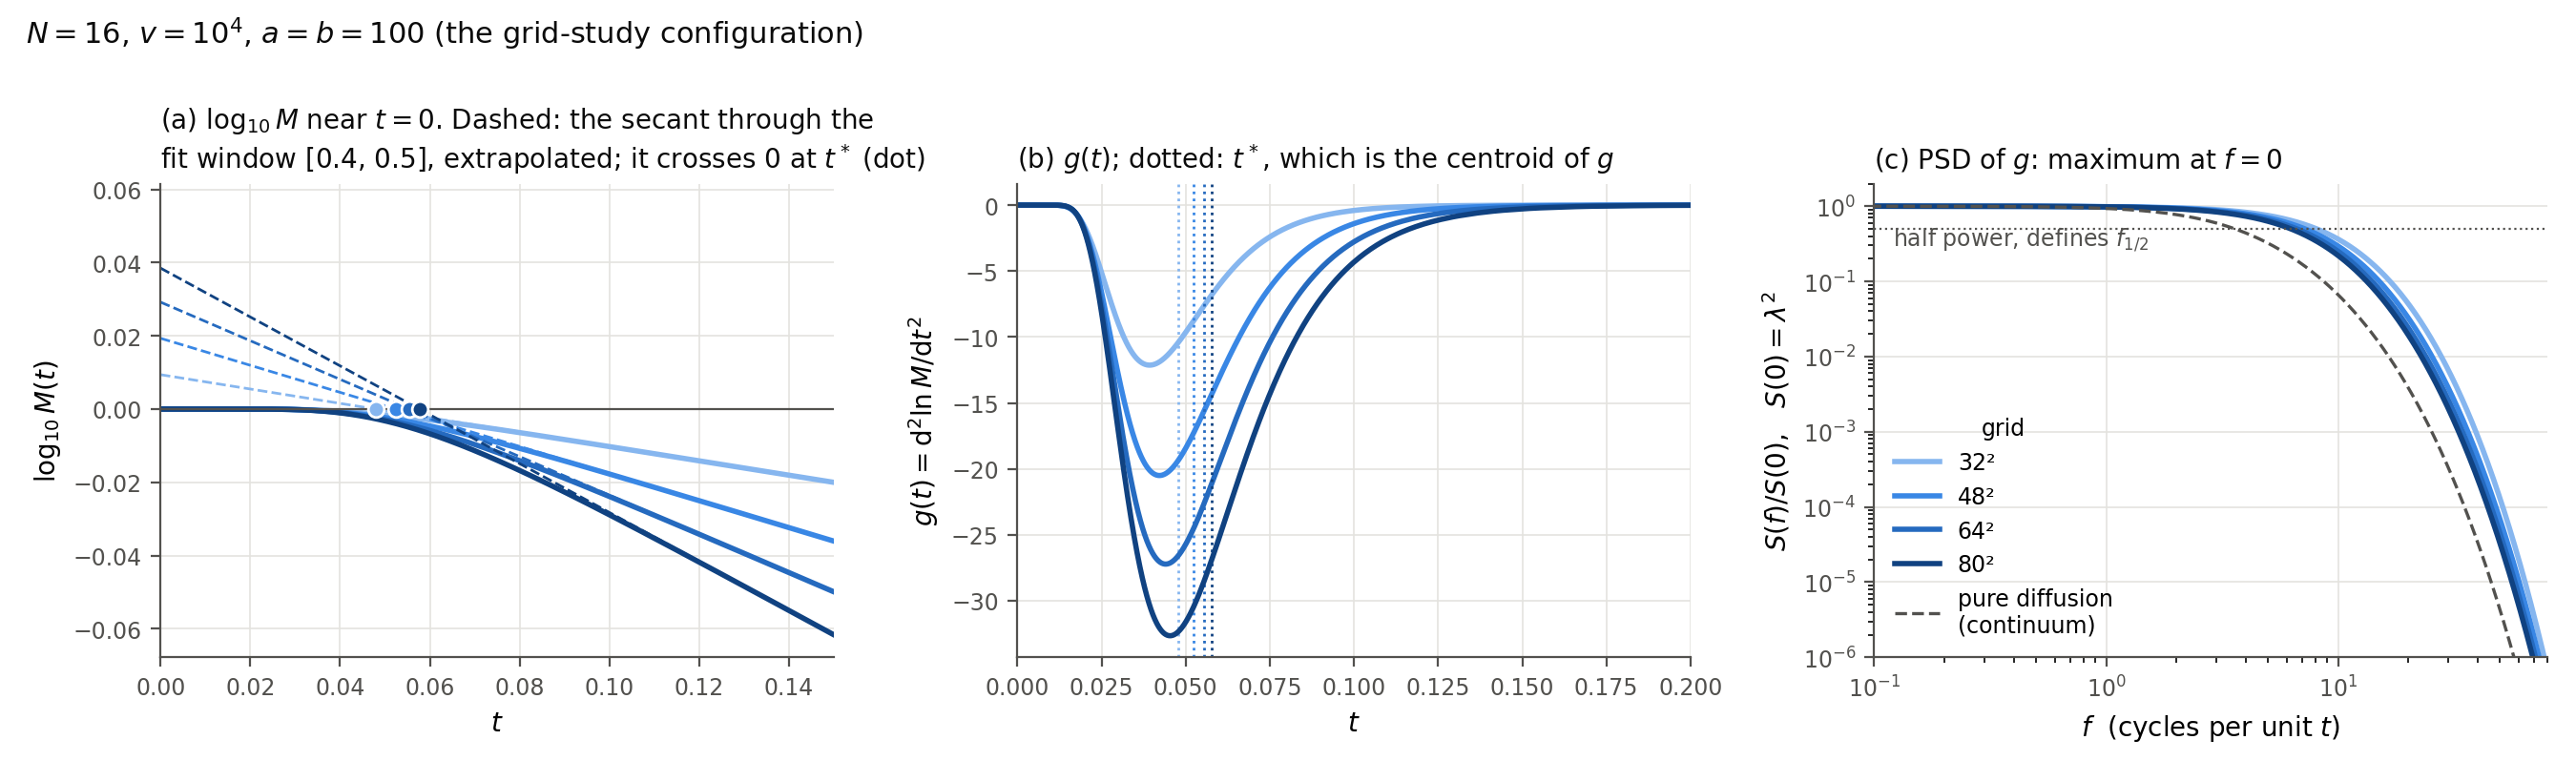
\includegraphics[width=\textwidth]{anatomy_grid_study_config.png}
\caption{The grid-study configuration ($N=16$, $v=10^4$, $a=b=100$, $T=1$) at
four resolutions. (a) The $\tsec$ construction. (b) $g$ is a single negative pulse
with $\tsec$ (dotted) at its centroid. (c) Its PSD, normalised by $S(0)=\lambda^2$,
peaks at $f=0$. Dashed: continuum pure diffusion.}
\label{fig:anatomy}
\end{figure}

\begin{table}[H]
\centering
\small
\input{\tabdir/table_identities.tex}
\caption{The exact results, checked on the 49 runs of the sweep. The
window-weighted form \eqref{eq:window} and the secant are evaluated at the same
two samples, so they agree to rounding. The plain centroid \eqref{eq:centroid}
deviates most when decay is slowest, where $g$ has not quite died out by
$t=0.4$.}
\label{tab:identities}
\end{table}

\begin{figure}[H]
\centering
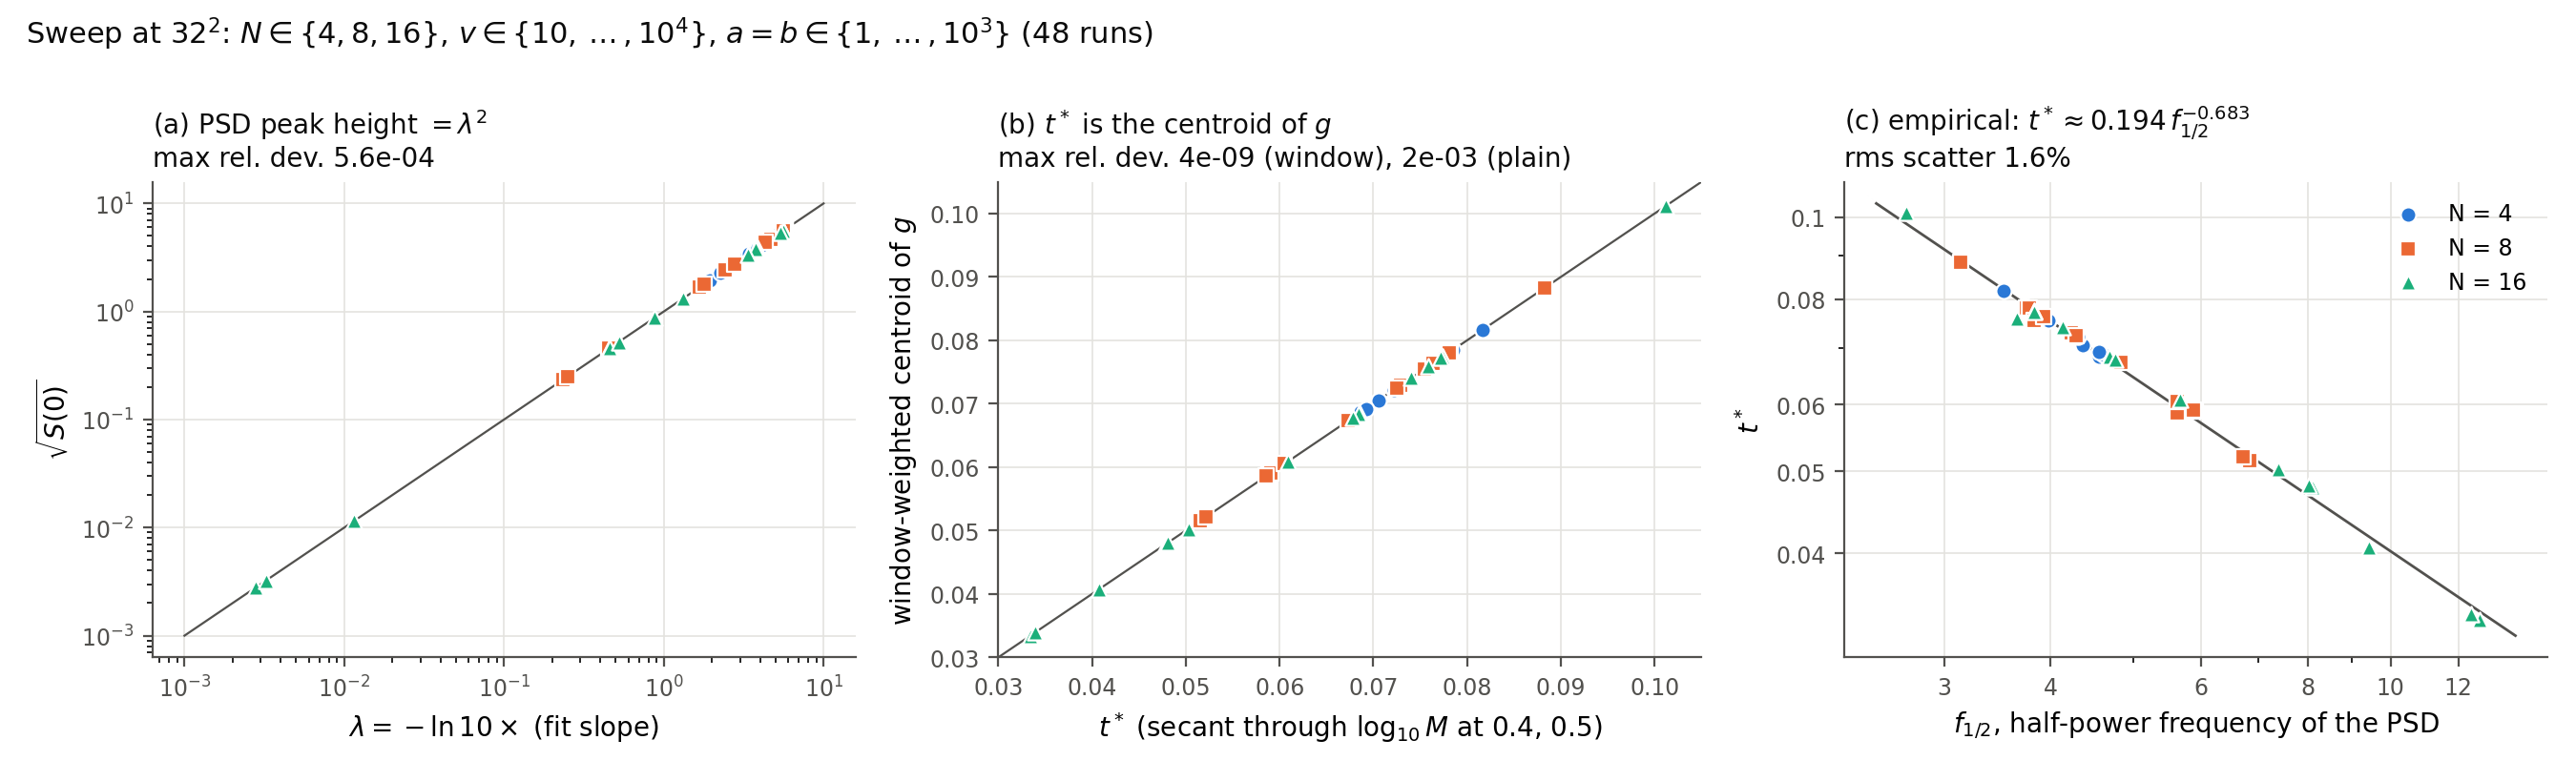
\includegraphics[width=\textwidth]{sweep_identities.png}
\caption{The sweep. (a) $\sqrt{S(0)}=\lambda$. (b) $\tsec$ equals the
window-weighted centroid of $g$. (c) The empirical link between $\tsec$ and the
PSD's half-power frequency.}
\label{fig:sweep}
\end{figure}

\paragraph{The empirical link to the PSD width.}
Across the sweep, $\tsec\approx0.194\,f_{1/2}^{-0.683}$, with 1.6\% rms scatter in
$\ln\tsec$ and a worst case of 5.7\%. The product $\tsec f_{1/2}$ ranges from 0.274
to 0.425 (0.295 for continuum diffusion). It is largest where active transport is
strongest ($N=16$, $a=b=10^3$, $v\ge10^3$). There the escape rate switches on more
sharply relative to its delay: $\tsec/\sigma$ reaches 3.0, against 1.92 for
diffusion. This is a correlation within the family, not a law: $R=D=1$
throughout, so the prefactor carries hidden units.

\begin{table}[H]
\centering
\small
\input{\tabdir/table_grid.tex}
\caption{The grid-study configuration under refinement. $\lambda$ and $\tsec$
show the same non-convergence documented in the 2026-08-18 study, and the
spectral quantities inherit it. The identities hold exactly at every grid.}
\label{tab:grid}
\end{table}

\section{Results II: the $(a,b)$ grid of the current studies}
\label{sec:ab}

The current $t^*$ studies use $v=1$ and $N=4$, with $(a,b)\in\{0.1,1,10,100\}^2$.
We ran all sixteen pairs at $32^2$ to $T=6$, long enough for every pair to settle
at $\tau=10^{-3}$, and the $b=0.1$ column again at $48^2$.

\begin{figure}[H]
\centering
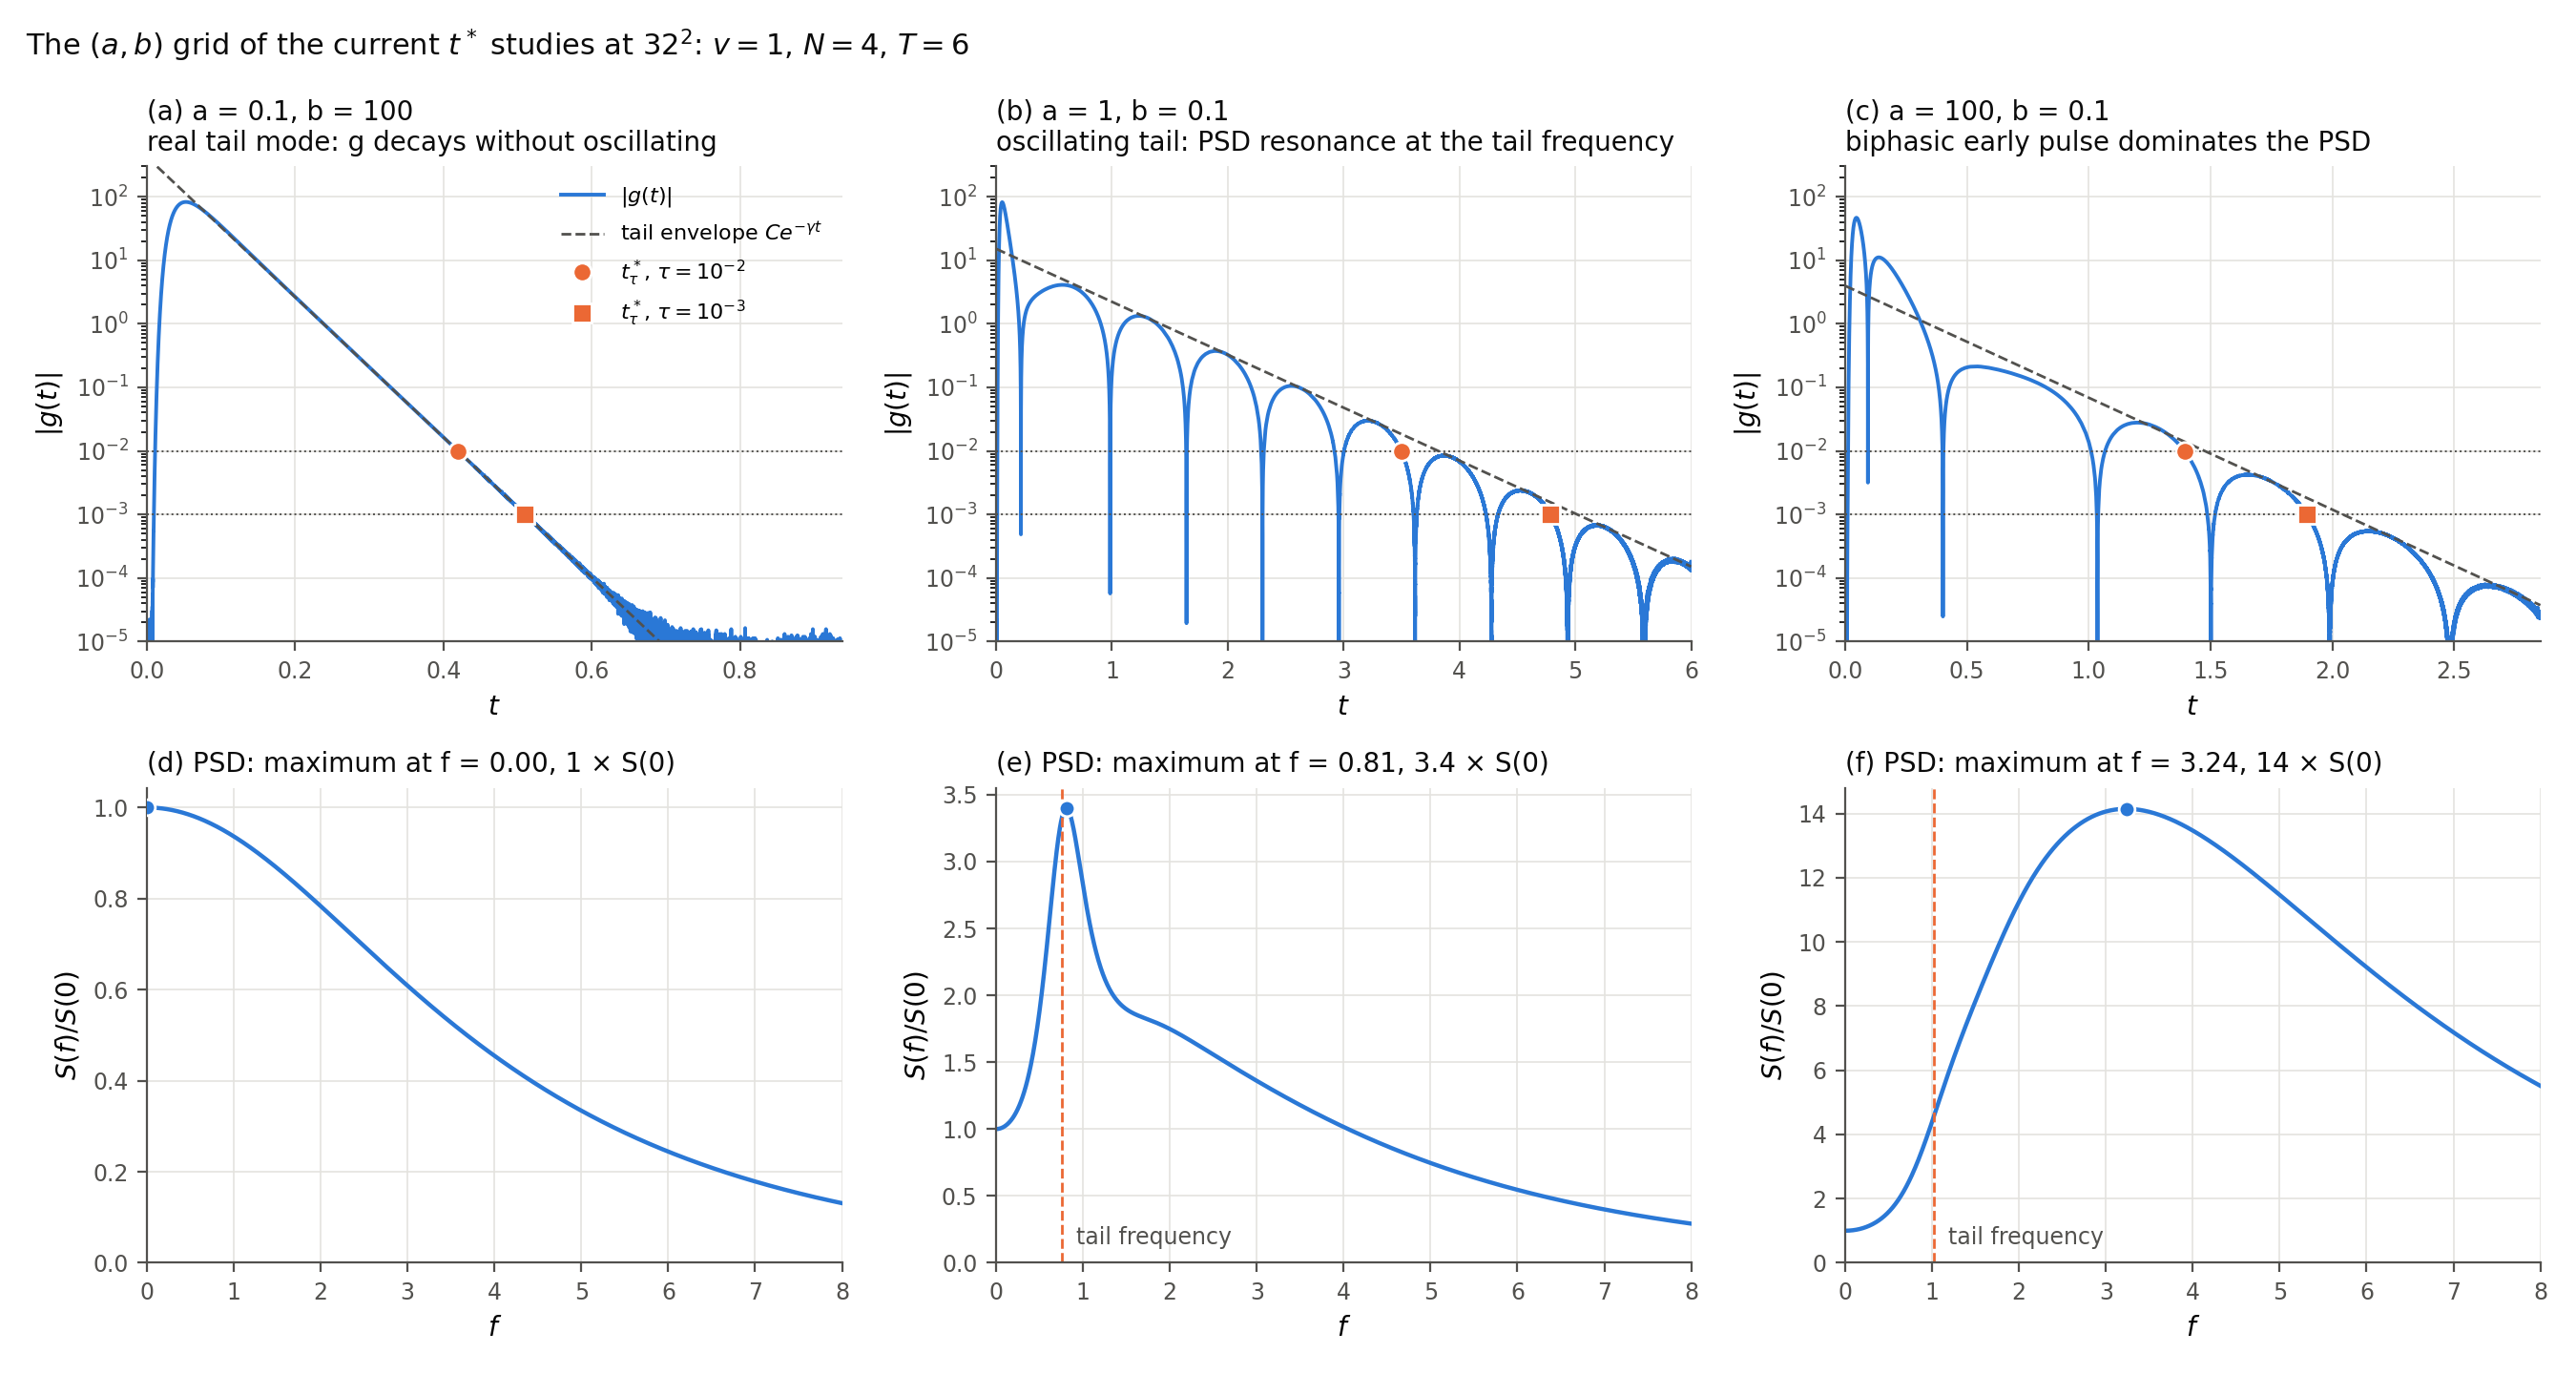
\includegraphics[width=\textwidth]{ab_examples.png}
\caption{Three regimes. (a, d) $b=100$: $g$ decays without oscillating, the PSD
peaks at $f=0$, and $\ttau$ lies exactly on the envelope. (b, e) $a=1$, $b=0.1$:
a long damped oscillation; the PSD resonance sits at the tail frequency, and
$\ttau$ falls within half a period of the envelope crossing. (c, f) $a=100$,
$b=0.1$: a fast biphasic pulse dominates the PSD ($14\,S(0)$ at $f=3.24$), while
the tail, which sets $\ttau$, oscillates at $f=1.02$.}
\label{fig:abex}
\end{figure}

\begin{table}[H]
\centering
\footnotesize
\setlength{\tabcolsep}{3.5pt}
\input{\tabdir/table_ab.tex}
\caption{The $(a,b)$ grid at $32^2$. Column key:
\textit{tail} is the type of the slowest tail mode (real; oscillating;
\textit{two} close modes). $p$ is the positive fraction of $g$.
$f_{\max}$ and $S_{\max}$ are the location and height of the PSD maximum.
$\omega/2\pi$ and $\gamma$ are the tail mode from the matrix pencil, and
$\gamma_\tau=[\dd\ttau/\dd\ln(1/\tau)]^{-1}$. $t_{\rm env}=\ln(C/\tau)/\gamma$ is
given for $\tau=10^{-2}$ and $10^{-3}$. $\tsec$ is the original definition.
$S(0)=\lambda^2$ holds against the current kernel's slope to
$7\times10^{-6}$ in all sixteen pairs, and \eqref{eq:window} reproduces $\tsec$ to
$6\times10^{-9}$, negative values included. The bound \eqref{eq:bound} holds for
every pair.}
\label{tab:ab}
\end{table}

\begin{figure}[H]
\centering
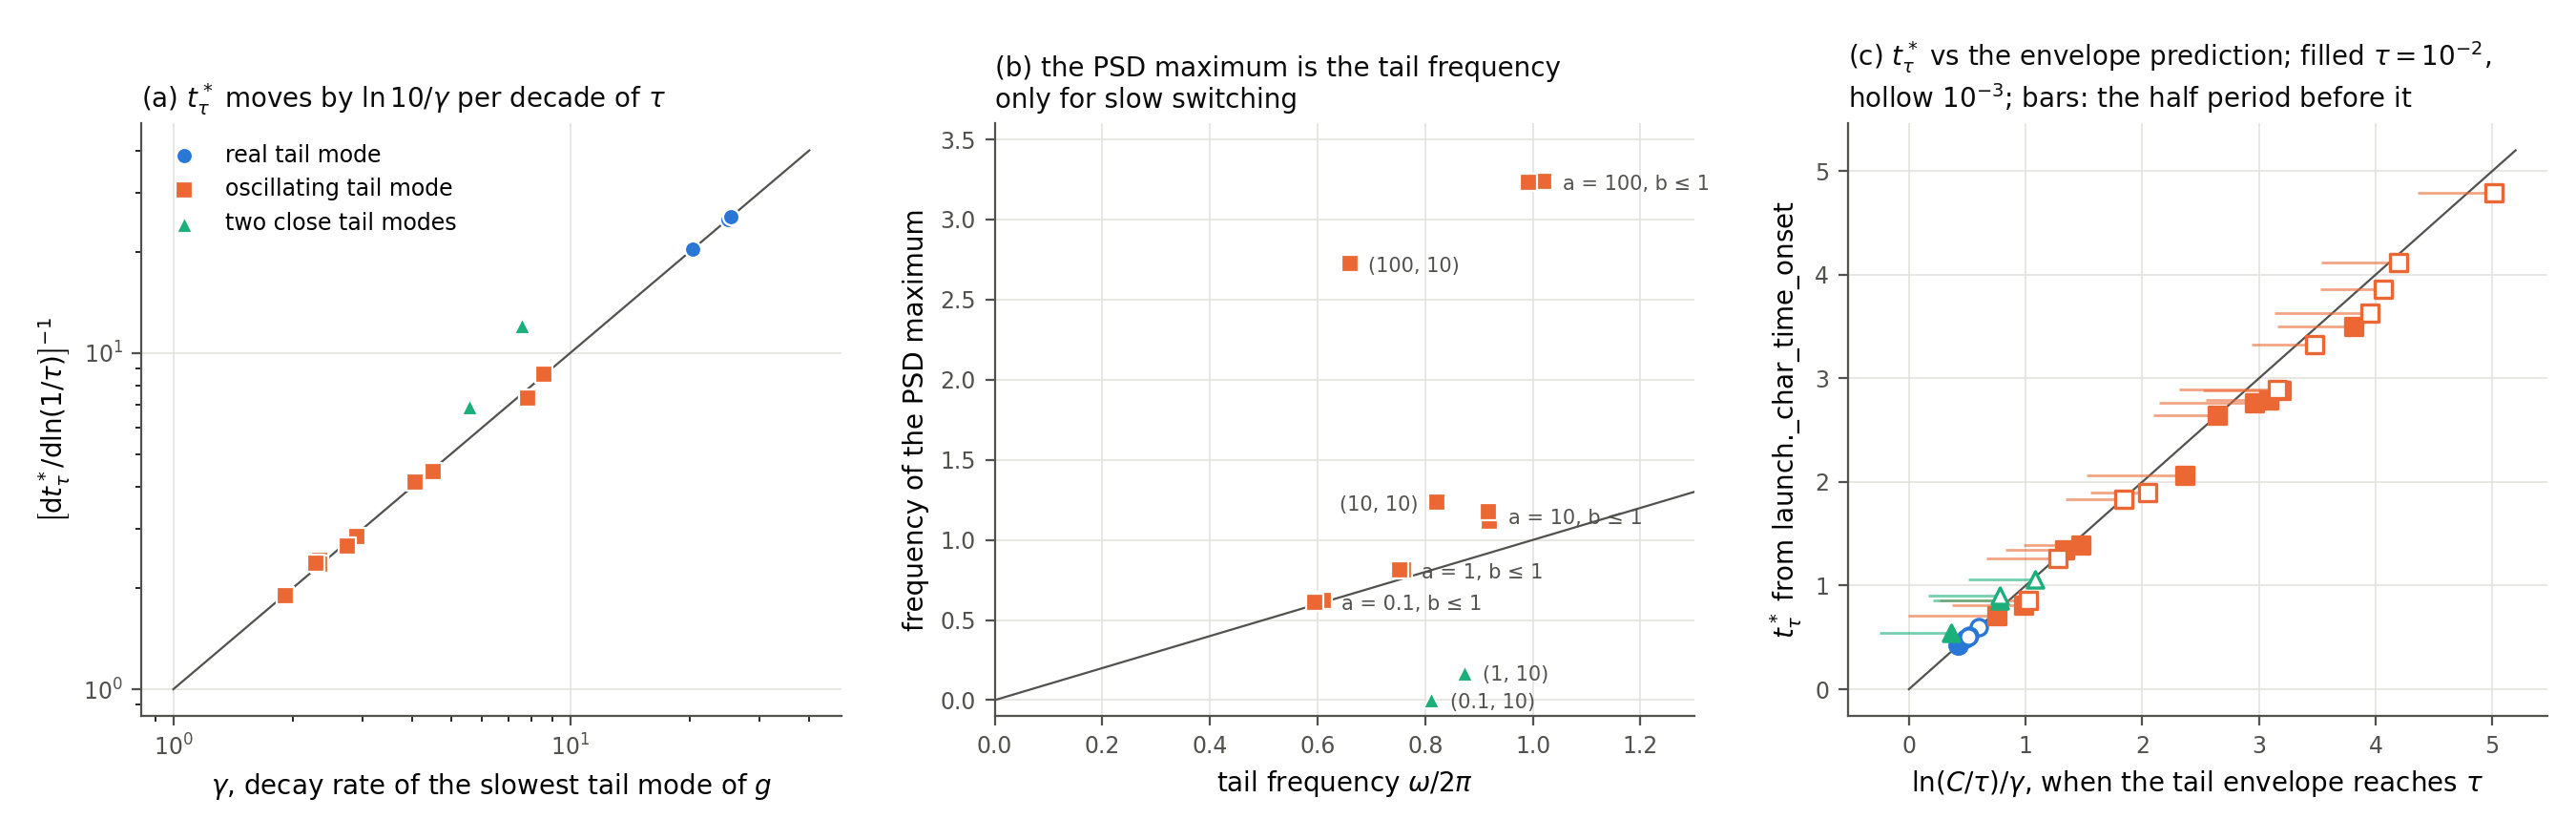
\includegraphics[width=\textwidth]{ab_relations.png}
\caption{(a) The $\tau$-sensitivity of $\ttau$ against the decay rate of the tail
mode, which tests \eqref{eq:tausens}. (b) The frequency of the PSD maximum against
the tail frequency. (c) $\ttau$ from the project's kernel against the envelope
prediction; bars span the half period before $t_{\rm env}$.}
\label{fig:abrel}
\end{figure}

\paragraph{The current $t^*$.}
\begin{itemize}
\item \textbf{Real tail modes} (the four $b=100$ pairs): $\gamma_\tau$ equals
  $\gamma$ to 0.09\%, and $\ttau=t_{\rm env}$ to the third decimal at both
  thresholds. The relation $\ttau=\ln(C/\tau)/\gamma$ is exact here.
\item \textbf{Oscillating tail modes} (ten pairs): $\gamma_\tau$ is within 6.3\%
  of $\gamma$. In 19 of 20 cases (ten pairs, two thresholds),
  $t_{\rm env}-\ttau$ lies between 0 and the half period $\pi/\omega$; the 20th
  overshoots by 0.007.
\item \textbf{Two close modes} ($b=10$ with $a\le1$): a complex pair and a real
  mode decay at similar rates and beat against each other. The single-mode
  description does not apply ($\gamma_\tau$ is off by 25--60\%), though $\ttau$
  is still within $0.18$ of $t_{\rm env}$.
\end{itemize}

\paragraph{The PSD peak.}
For every pair with $b\ge10$ and $a\le10$, apart from $(10,10)$, $g$ is
essentially single-signed and the PSD peaks at or very near $f=0$. With $b\le1$
there are two separate sources of positive $g$:
\begin{itemize}
\item a \emph{late damped oscillation} of the escape rate, which gives a narrow
  resonance at the tail frequency;
\item an \emph{early overshoot}, which makes the initial pulse biphasic and gives
  a broad band-pass hump at $f\sim1/(\text{pulse duration})$.
\end{itemize}
For $a\le1$ the resonance dominates, and $f_{\max}$ equals $\omega/2\pi$ to within
2--8\%. At $a=10$ (still with $b\le1$) the two are comparable, and $f_{\max}$ sits 21--28\% above the
tail frequency. At $a=100$ the early pulse dominates, and $f_{\max}=3.2$ against a
tail at $1.0$. Only the resonance bears on $\ttau$, through
\eqref{eq:tausens}. We did not measure $\gamma$ from the resonance width, because
the resonance rides on the broadband shoulder of the pulse (Fig.~\ref{fig:abex}e).
The tail of $g$ gives $\gamma$ more cleanly.

\begin{table}[H]
\centering
\small
\input{\tabdir/table_ab_grid.tex}
\caption{The $b=0.1$ column at $32^2$ and $48^2$. The values move with the grid,
as every quantity in this project does, but the relations between them do not:
$\gamma_\tau\approx\gamma$, $\ttau$ falls just before $t_{\rm env}$, and $f_{\max}$
departs from $\omega/2\pi$ as $a$ grows.}
\label{tab:abgrid}
\end{table}

\section{Caveats}
\begin{itemize}
\item \textbf{Off-the-shelf estimators show a false peak.} On $g$ over $[0,1]$,
  \path{scipy.signal.periodogram} peaks at $f=1/T$. Its one-sided convention
  doubles every bin except DC, so the first nonzero bin outscores DC whenever it
  lies well inside the flat top of the spectrum. \path{scipy.signal.welch} with
  default settings also removes the mean, which zeroes DC outright; it peaks at
  its first nonzero frequency bin, $f_s/n_{\rm perseg}$. Both peaks move with $T$
  or the segment length, so neither is physical. Use the two-sided $|G(f)|^2$.
\item \textbf{Assumptions.} The identities need $M(0)=1$ and $\kappa(0)=0$. An
  off-centre initial condition next to the rim breaks $\kappa(0)=0$; then
  $\tsec=\int tg/(\int g-\kappa(0))$.
\item \textbf{Resolution.} The $(a,b)$ results are at $32^2$, with a check at
  $48^2$. Values of $\ttau$ differ from the $96^2$ study (for example
  $\ttau(10^{-2})$ is 3.50 at $32^2$ against 2.89 at $96^2$ for $(1,0.1)$), as
  expected from the documented grid dependence. The relations are structural and
  should carry over; the numbers will not.
\item \textbf{Limits of the modal picture.} It assumes one slowest correction
  mode. Where two modes are close, as in two pairs here, $\ttau$ inherits a
  beating pattern that a single $(\gamma,\omega)$ does not describe.
\end{itemize}

\section{Reproducing}
{\small
\begin{verbatim}
python scripts/psd_d2_ln_mass.py solve --set sweep  # 49 runs, ~2.5 min, 8 cores
python scripts/psd_d2_ln_mass.py solve --set grids  # 32^2-80^2; 80^2 ~30 min
python scripts/psd_d2_ln_mass.py solve --set ab     # 16 pairs at 32^2, 4 at 48^2
python scripts/psd_d2_ln_mass.py report             # CSVs, figures, tables
cd findings && tectonic psd_d2_ln_mass_report.tex
\end{verbatim}}
Raw $M(t)$ series are written to \path{data_output/psd_d2_ln_mass/raw/}.
Figures, the per-run metrics (\path{psd_metrics.csv}, \path{ab_metrics.csv}) and the
table fragments are in \path{results/2026-10-15_psd-d2-ln-mass/}.

\end{document}
